\documentclass[12pt]{article}
\usepackage{amsmath,amsfonts,amsthm,amssymb}
\usepackage{setspace}
\usepackage{fancyhdr}
\usepackage{lastpage}
\usepackage{extramarks}
\usepackage[ruled,vlined]{algorithm2e}
\usepackage{chngpage}
\usepackage{soul,color}
\usepackage{graphicx,float,wrapfig}
\usepackage{ listings}
\usepackage{enumitem}
\newcommand{\Class}{\normalsize CS 370: Introduction to Computational Geometry}
%\newcommand{\ClassInstructor}{Fares}
% Homework Specific Information. Change it to your own
\newcommand{\Title}{Assignment 2}
\newcommand{\StudentName}{Brady Zhou}
\newcommand{\StudentClass}{50705}
\newcommand{\StudentNumber}{bz2459}

% In case you need to adjust margins:
\topmargin=-0.45in      %
\evensidemargin=0in     %
\oddsidemargin=0in      %
\textwidth=6.5in        %
\textheight=9.0in       %
\headsep=0.25in         %

% Setup the header and footer
\pagestyle{fancy}                                                       %
\lhead{\StudentName}                                                 %
\rhead{\firstxmark}                                                     %
\lfoot{\lastxmark}                                                      %
\cfoot{}                                                                %
\rfoot{Page\ \thepage\ of\ \protect\pageref{LastPage}}                          %
\renewcommand\headrulewidth{0.4pt}                                      %
\renewcommand\footrulewidth{0.4pt}                                      %

\title{\textmd{\bf \Class\\}}
\author{\small \normalfont{Advisor: Chandrajit Bajaj}\\
\small \normalfont{\StudentName}}

\date{} 
\begin{document}
\maketitle \thispagestyle{empty}

\subsection{Turn Orientation}

\quad\qquad A key recurring theme in computation is the problem of floating point error. A common tool in the geometry toolbox is the idea of \textbf{turn orientation}, that is, whether a set of three points makes a clockwise (right), or counter-clockwise (left) turn. In a naive implementation of determining orientation of a turn, the angle of the line formed is calculated using some form of division and arcos. This can lead to loss of precision due to floating point numbers.

\quad A better way to deal with line orientation is to take the determinant of the three points and if the determinant is larger than some $\epsilon$, the points make a clockwise turn. If the determinant falls within $-\epsilon$ to $\epsilon$, we say the points are colinear, and if the determinant is smaller than $\epsilon$, the points make a counter-clockwise turn. This implementation is faster in the sense it does not use division, and more robust. \newline 
\\
\centerline{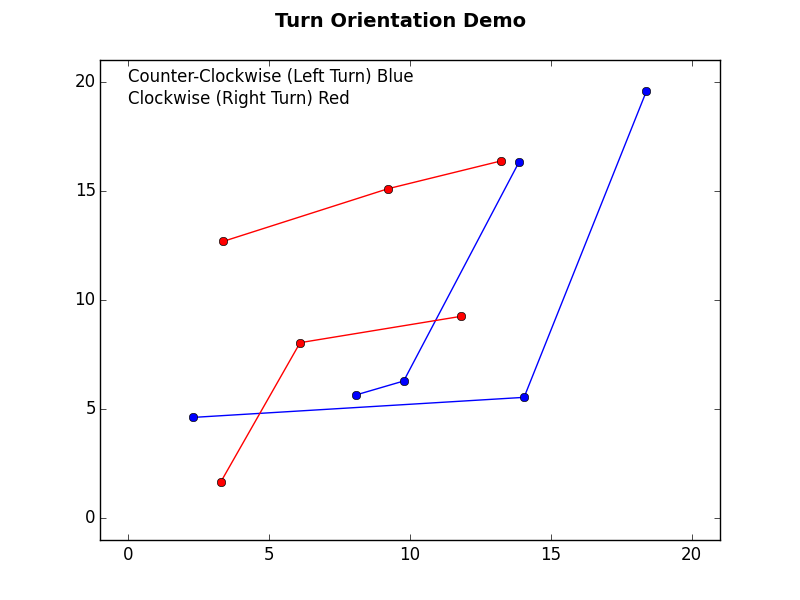
\includegraphics[scale=0.7]{turn_orientation.png}}

\subsection{Convex Hull}


\end{document}
